\section{Betriebsverhalten}
\subsection{Natürliche Leistung}
    \begin{itemize}
        \item Bei einer gewissen Belastung wird in den Querelementen genau so viel Blindleistung „erzeugt“ wie im Längspfad „verbraucht“ wird.
        \item Diese Belastung nennt man natürliche Belastung bzw. natürliche Leistung.
        \item Die Leitung verhält sich neutral bezüglich Blindleistung.
        \item Die natürliche Leistung wird übertragen, wenn die Leitung mit ihrer Wellenimpedanz belastet wird.
    \end{itemize}

    \vspace{0.1cm}

    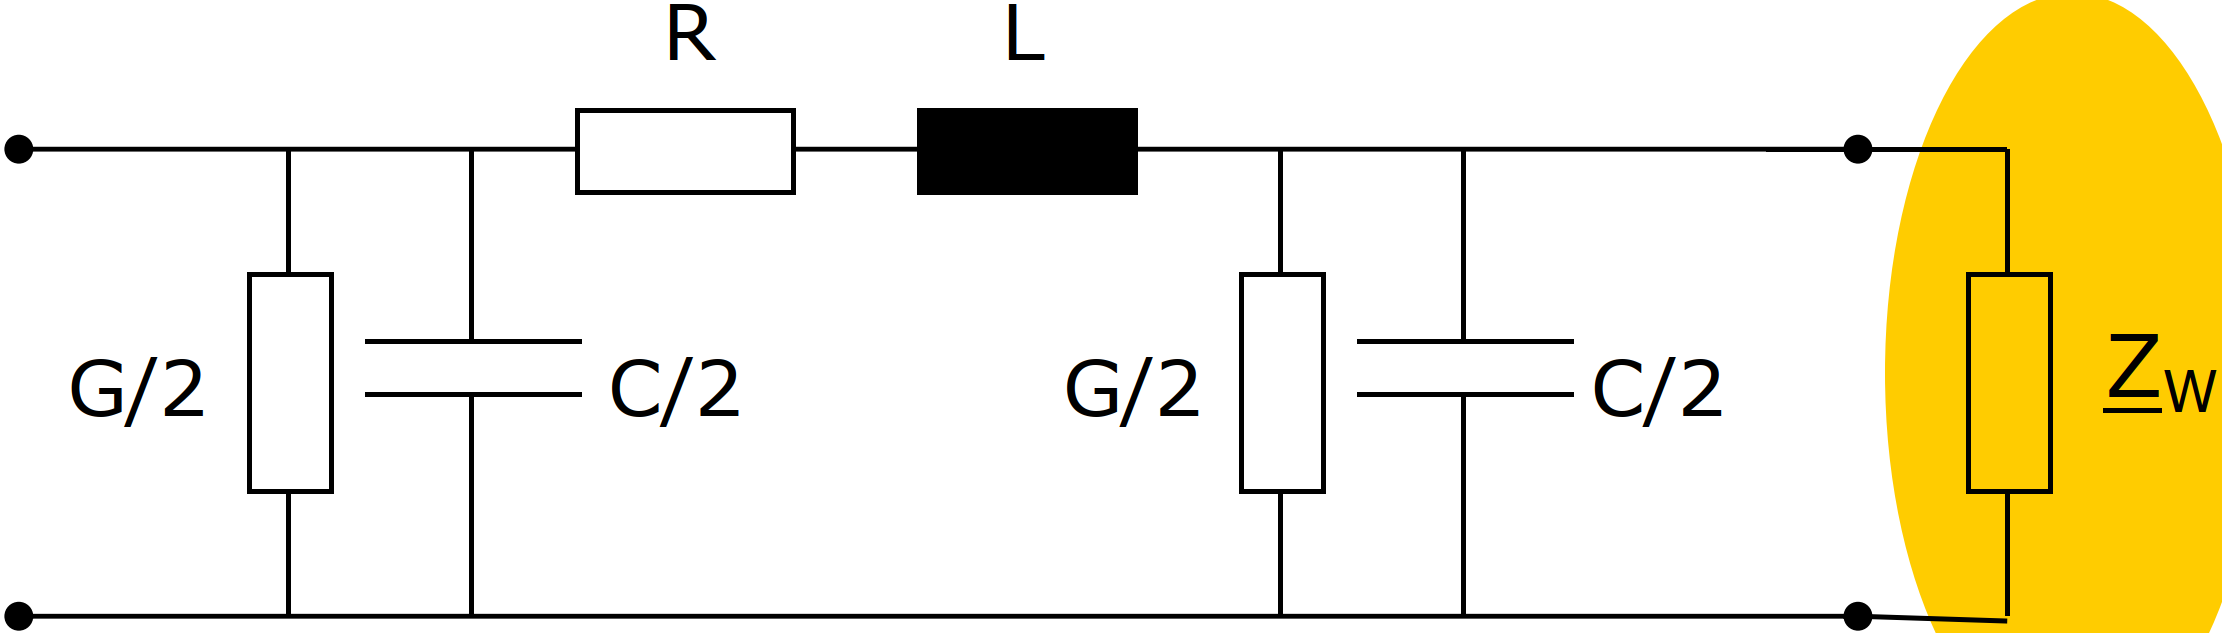
\includegraphics[width=0.9\columnwidth, align=c]{images/Natürliche_Leistung.png}

\subsection{Wellenimpedanz}
    \begin{itemize}
        \item Bei Abschluss mit der Wellenimpedanz „erzeugt“ die Leitung genau so viel Blindleistung wie sie „verbraucht“.
        \item Typische Wellenimpedanzwerte für Freileitung: \( |\!Z_W\!| = 200 \ldots 400\,\Omega \).
        \item Typische Wellenimpedanzwerte für Kabel: \( |\!Z_W\!| = 30 \ldots 50\,\Omega \).
    \end{itemize}

\subsection{Unternatürliche Belastung}
    \begin{itemize}
        \item Die Lastimpedanz ist höher als die Wellenimpedanz.
        \item Die Last nimmt weniger als die natürliche Leistung auf, Leitung nimmt Blindleistung auf.
        \item Die Längsinduktivität „verbraucht“ weniger Blindleistung als die Quer­kapazität „erzeugt“.
        \item Die Spannung am Leitungsende ist höher als am Leitungsanfang.
    \end{itemize}

\subsection{Übernatürliche Belastung}
    \begin{itemize}
        \item Die Lastimpedanz ist niedriger als die Wellenimpedanz.
        \item Die Last nimmt mehr als die natürliche Leistung auf, Leitung gibt Blindleistung ab.
        \item Die Längsinduktivität „verbraucht“ mehr Blindleistung als die Quer­kapazität „erzeugt“.
        \item Die Spannung am Leitungsende ist tiefer als am Leitungsanfang.
    \end{itemize}

\subsection{Praxis}
    \begin{itemize}
        \item \textbf{Kabel} ausschließlich \textbf{unternatürlich} betrieben
        \item \textbf{Freileitungen} meistens \textbf{unternatürlich} betrieben, in seltenen Fällen \textbf{übernatürlich}
    \end{itemize}

\subsection{Leerlauf}
    \begin{minipage}[t]{0.59\columnwidth}
        \begin{itemize}
            \item Extremfall der unternatürlichen Belastung
            \item Leitung verhält sich wie Kapazität
            \item Spannung steigt entlang der Leitung an
            \item Spannungsüberhöhung am Leitungsende 
            \item[] (Ferranti Effekt)
        \end{itemize}
    \end{minipage}%
    \hfill
    \begin{minipage}[t]{0.4\columnwidth}
        % \vspace{0.1cm}
        \centering \vspace{-0.7\baselineskip}
        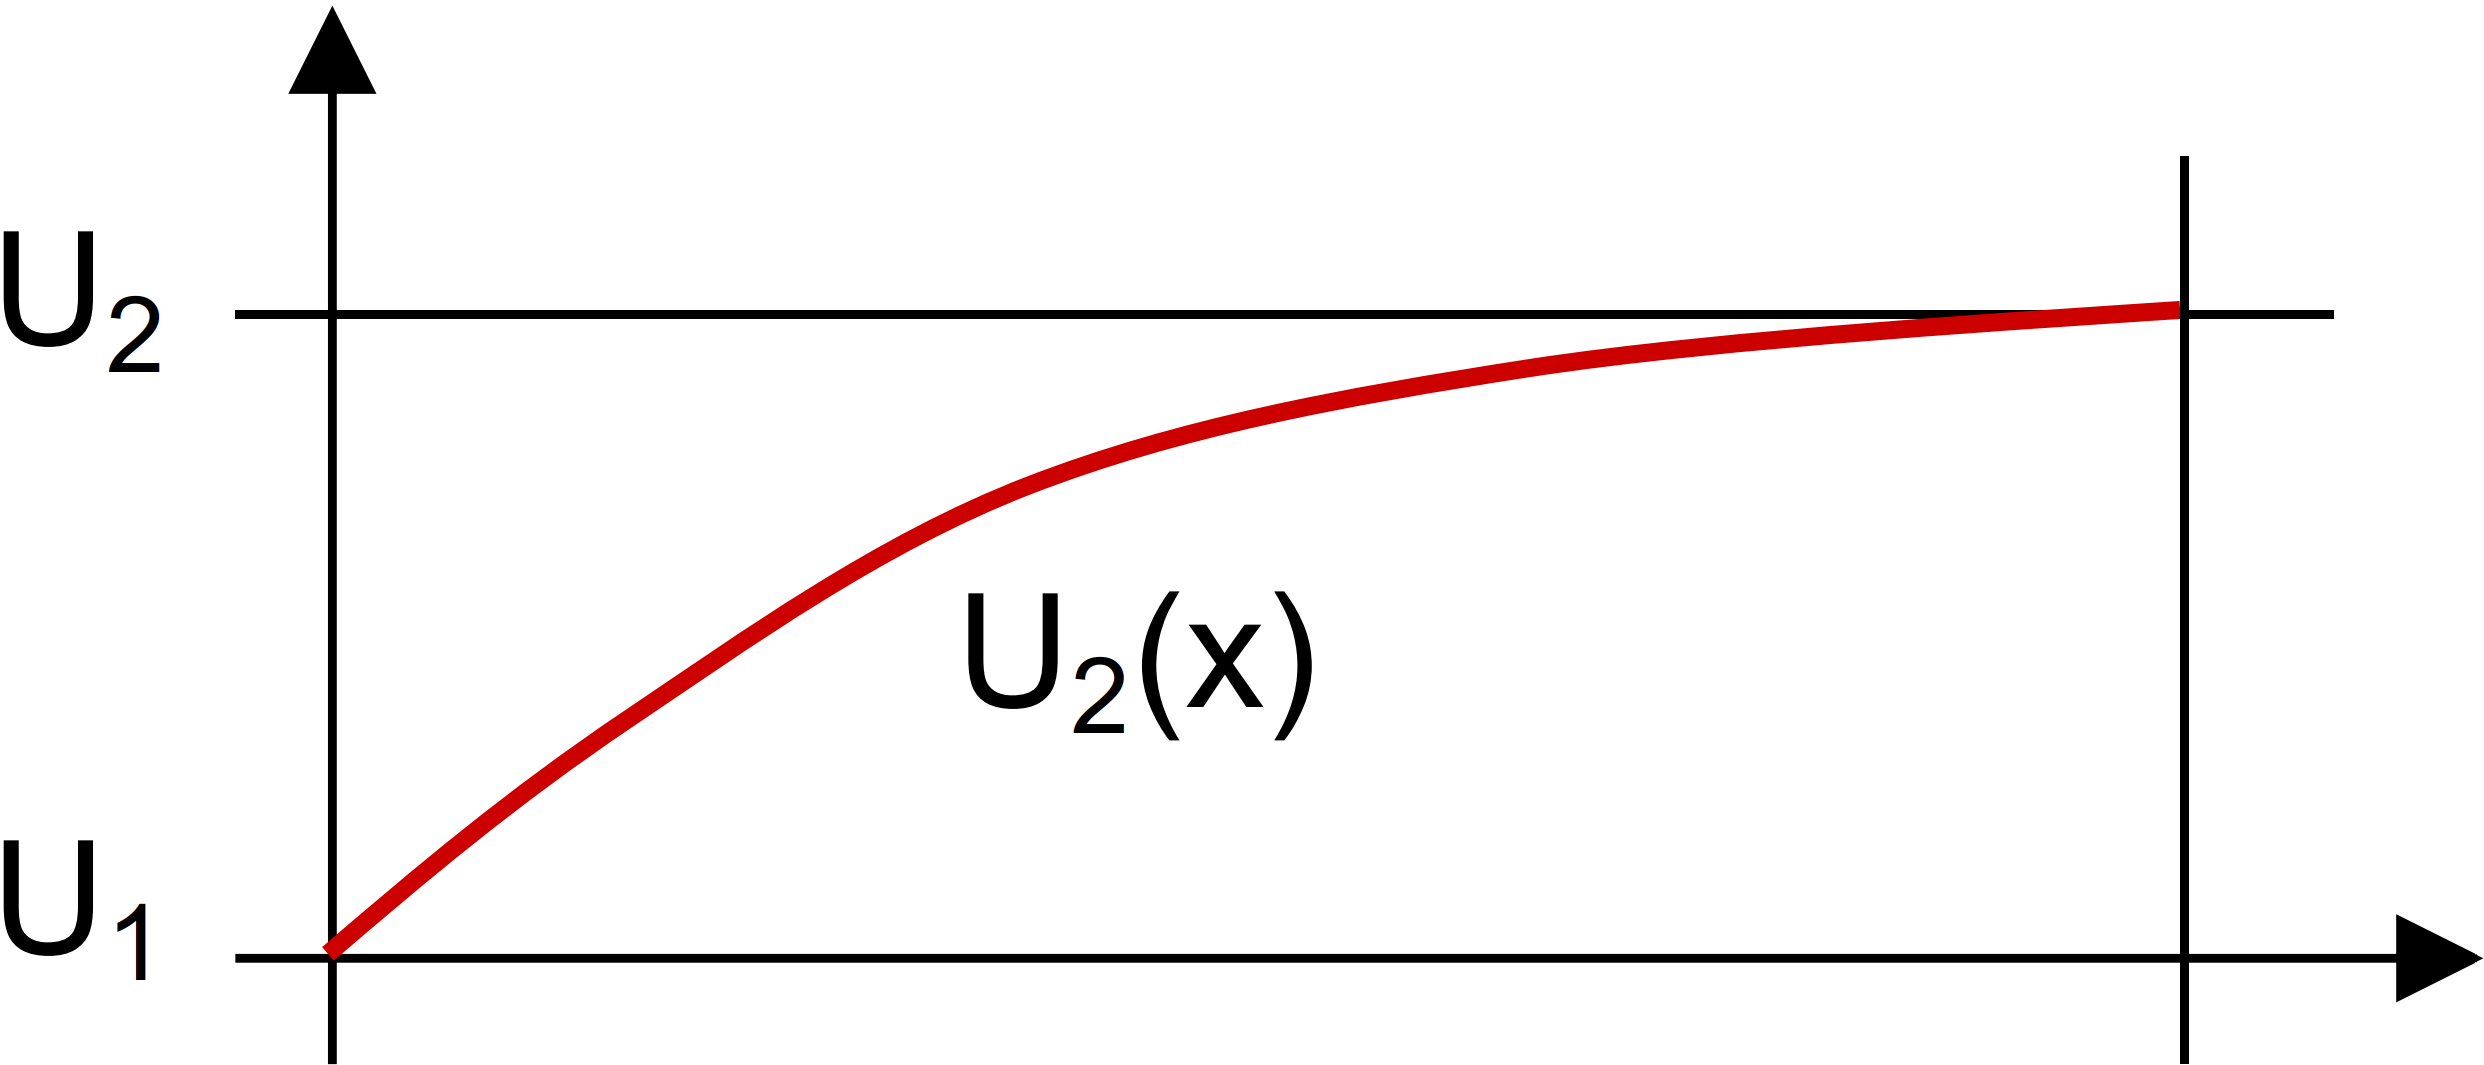
\includegraphics[width=0.9\columnwidth, align=c]{images/Leerlauf.png}
    
        % \vspace{0.1cm}
    \end{minipage}


\subsection{Kurzschluss}
    \begin{itemize}
        \item Extremfall der übernatürlichen Belastung
        \item Leitung verhält sich wie Induktivität
        \item Spannung sinkt entlang der Leitung ab
    \end{itemize}

\subsection{Spannungsabfall entlang einer Leitung}
    \begin{minipage}[t]{0.55\columnwidth}
        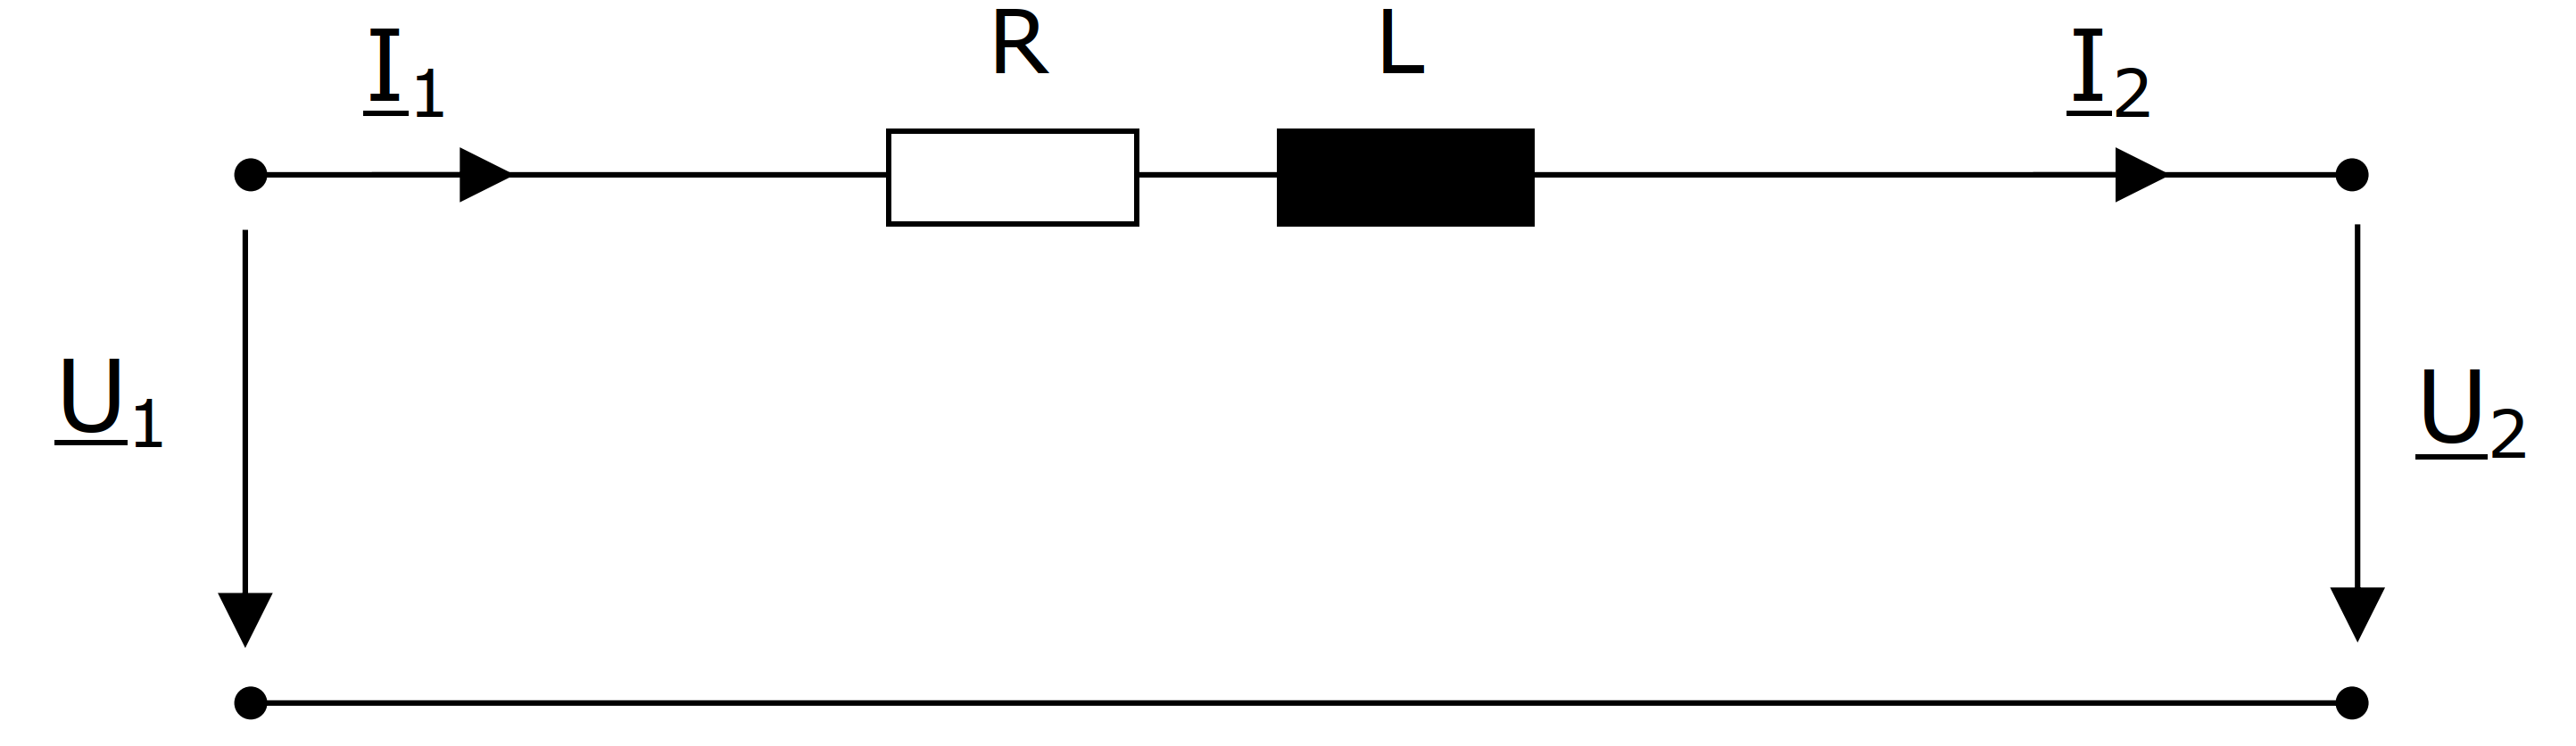
\includegraphics[width=0.95\columnwidth, align=c]{images/Spannungsabfall_entlang_einer_Leitung.png}
    \end{minipage}%
    \hfill
    \begin{minipage}[t]{0.4\columnwidth}
        % \centering \vspace{-0.7\baselineskip}
        \resizebox{!}{0.3\textwidth}{% \begin{figure}[!ht]
% \centering
% \resizebox{1\textwidth}{!}{%
\begin{circuitikz}
\tikzstyle{every node}=[font=\fontsize{18pt}{18pt}\selectfont]
\draw [-{Stealth[scale=1.5]}] (3.75,9) -- (10,9)node[pos=0.5, below, text opacity=1, inner xsep=0.080cm, inner ysep=0.085cm, rounded corners=0.020cm]{$\underline{U}_2$};
\draw [-{Stealth[scale=1.5]}] (10,9) -- (12.5,7.75)node[pos=0.5, below, text opacity=1, inner xsep=0.080cm, inner ysep=0.085cm, rounded corners=0.020cm]{$R\underline{I}_2$};
\draw [-{Stealth[scale=1.5]}] (3.75,9) -- (5,8.375)node[pos=0.5, below, text opacity=1, inner xsep=0.080cm, inner ysep=0.085cm, rounded corners=0.020cm]{$\underline{I}_2$};
\draw [-{Stealth[scale=1.5]}] (12.5,7.75) -- (14.25,11.375)node[pos=0.5, right, text opacity=1, inner xsep=0.080cm, inner ysep=0.085cm, rounded corners=0.020cm]{$jX\underline{I}_2$};
\draw [-{Stealth[scale=1.5]}] (3.75,9) -- (14.25,11.375)node[pos=0.5, above, text opacity=1, inner xsep=0.080cm, inner ysep=0.085cm, rounded corners=0.020cm]{$\underline{U}_1$};
\end{circuitikz}
% }%
% \caption{Your Caption}
% \label{fig:my_label}
% \end{figure}\unskip}
    \end{minipage}


\subsubsection{Phasenstrom durch Leitung}
    $
    \boxed{
    I_{Phase} = \frac{U_{Phase}}{Z_{Phase}}
    }
    $

    \vspace{0.1cm}